%%%%%%%%%%%%%%%%%%%%%%%%%%%%%%%%%%%%%%%%%
% a0poster Portrait Poster
% LaTeX Template
% Version 1.0 (22/06/13)
%
% The a0poster class was created by:
% Gerlinde Kettl and Matthias Weiser (tex@kettl.de)
% 
% This template has been downloaded from:
% http://www.LaTeXTemplates.com
%
% License:
% CC BY-NC-SA 3.0 (http://creativecommons.org/licenses/by-nc-sa/3.0/)
%
%%%%%%%%%%%%%%%%%%%%%%%%%%%%%%%%%%%%%%%%%

%----------------------------------------------------------------------------------------
%	PACKAGES AND OTHER DOCUMENT CONFIGURATIONS
%----------------------------------------------------------------------------------------

\documentclass[a0,portrait]{a0poster}
\usepackage[utf8]{inputenc}%
\usepackage{multicol} % This is so we can have multiple columns of text side-by-side
\columnsep=60pt % This is the amount of white space between the columns in the poster
\columnseprule=0pt % This is the thickness of the black line between the columns in the poster

\usepackage[svgnames]{xcolor} % Specify colors by their 'svgnames', for a full list of all colors available see here: http://www.latextemplates.com/svgnames-colors
\xdefinecolor{tucol1}{rgb}{1.0 0.5 0.05}
\xdefinecolor{tucol2}{rgb}{0.52,0.72,0.10}
\xdefinecolor{tucol3}{rgb}{0.0 0.0 0.8}
\xdefinecolor{tucol4}{rgb}{0.8 0.8 0}
\xdefinecolor{tucol5}{rgb}{0.8 0 0.8}
\xdefinecolor{tucol6}{rgb}{0 0.8 0.8}
%\xdefinecolor{tucol7}{rgb}{0 0 0.8}
%\xdefinecolor{tucol8}{rgb}{0.8 0 0}
\usepackage{multirow}
\usepackage{times} % Use the times font
%\usepackage{palatino} % Uncomment to use the Palatino font

\usepackage[pdftex]{graphicx} % Required for including images
\graphicspath{{figures/}} % Location of the graphics files
\usepackage{booktabs} % Top and bottom rules for table
\usepackage[font=small,labelfont=bf]{caption} % Required for captions to tables and figures
\usepackage{amsfonts, amsmath, amsthm, amssymb} % For math fonts, symbols and environments
\usepackage{wrapfig} % Allows wrapping text around tables and figures
\usepackage{pgfplots}
\usepackage{bm}
\usepackage{enumitem}

\usepackage{pgfplots}
\usepackage{tikz}
\usetikzlibrary{arrows,positioning,shapes,automata,fit,calc,decorations.pathreplacing,angles,quotes,backgrounds}
\usetikzlibrary{spy}
\usepackage[export]{adjustbox}

\usepackage{booktabs}
\usepackage{tabularx}
\newcolumntype{L}[1]{>{\hsize=#1\hsize\raggedright\arraybackslash}X}
\newcolumntype{R}[1]{>{\hsize=#1\hsize\raggedleft\arraybackslash}X}
\newcolumntype{C}[1]{>{\hsize=#1\hsize\centering\arraybackslash}X}

% Table formatting
\usepackage{multirow}
\newcommand{\twolinecell}[2][c]{%
  \begin{tabular}[#1]{@{}c@{}}#2\end{tabular}}

%Define a poster section that writes in bold
\providecommand{\postersection}[1]{
\color{tucol2}
\section*{\sf \huge #1}\Large\sf
\color{Black}
}

% Set standard deviation to boldish
\pgfplotsset{
axis line style={line width=3pt},
/pgfplots/error bars/error bar style={line width=2pt},
/pgfplots/error bars/error mark options={rotate=90,black,mark size=10pt,line width=2pt},
}
\begin{document}


\sf\Huge\noindent\color{tucol2}\hspace*{-6.5mm}
\textbf{\MakeUppercase{Text Detection for Segmentation-free Wordspotting}}\color{Black}
\vspace*{15mm}


\noindent \begin{minipage}[b]{0.7\linewidth}
\huge\textbf{Eugen Rusakov and Gernot~A.~Fink\\
\large
(in collaboration with Leonard Rothacker, Sebastian Sudholt, and Matthias Kasperidus [1])
}\\[0.5cm] 
\Large
Department of Computer Science, TU Dortmund University, Germany
\end{minipage}
\begin{minipage}[t]{0.3\linewidth}
\hspace*{-2.9cm}

\includegraphics[width=20cm]{tud_logo_rgb.pdf}
\end{minipage}
\vspace*{-10mm}


\begin{multicols}{2}

\postersection{Abstract}
\vspace*{-10mm}
\noindent
The generation of word hypotheses for segmentation-free word spotting on document level is usually subject to
heuristic expert design. This involves strong assumptions about the visual appearance of text in the 
document images. 
The local region classificator generates detection scores, which are processed by a extremal region 
approach to generate hypotheses. Afterwards the Query is matched with the most similar hypotheses 
classified by the PHOCNet [1].~\\~\\~\\~\\

\columnbreak
%
\postersection{Historical Documents}
\vspace*{-10mm}

\begin{tikzpicture}[
	node distance = 5cm,
	auto,
	scale=1.0,
	transform shape,
	triangle/.style = {regular polygon, regular polygon sides=3 },
    node rotated/.style = {rotate=180},
    border rotated/.style = {shape border rotate=180}
	]
	
	\node[
	rounded corners=50pt,  
	%rectangle, draw, 
	minimum height=15cm, 
	minimum width=20cm] 
	(inside)
	at (0,0)
	{	};
	
	% Detector scores
	\node[rounded corners=10pt] at ([xshift=-7em, yshift=0em] inside.center) (lrc)
	{
		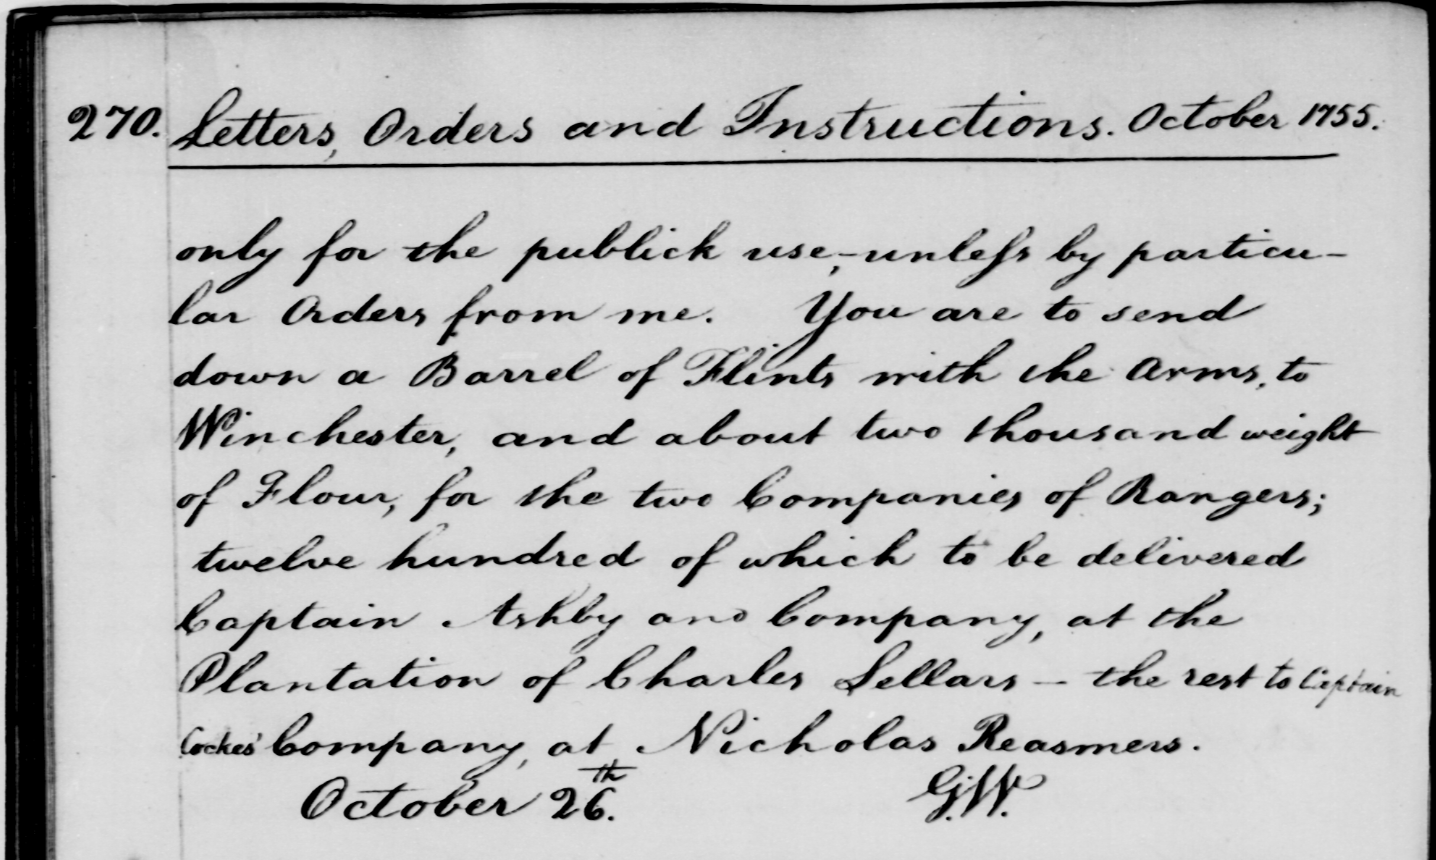
\includegraphics[width=20cm]{images/gw_page_example.png}
	};
	
	\node[rounded corners=10pt] at ([xshift=5em, yshift=3em] inside.center) (lrc)
	{
		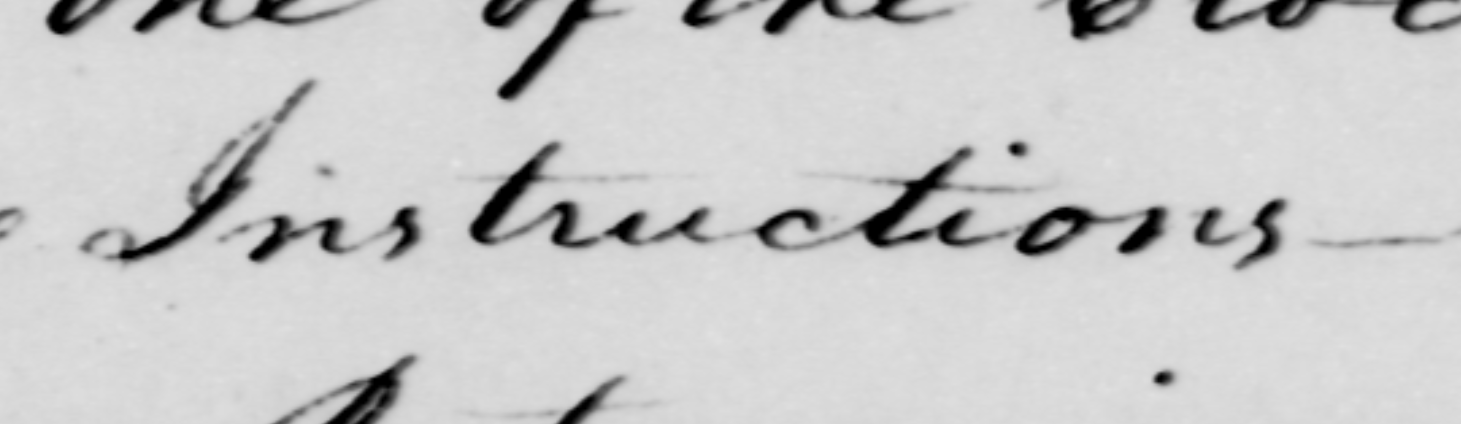
\includegraphics[width=8cm]{images/word_gap.png}
	};
	
	\node[rounded corners=10pt] at ([xshift=5em, yshift=0em] inside.center) (lrc)
	{
		
\includegraphics[width=8cm]{images/word_overlap.png}
	};
	
	\node[rounded corners=10pt] at ([xshift=5em, yshift=-3em] inside.center) (lrc)
	{
		
\includegraphics[width=8cm]{images/word_overline.png}
	};

\end{tikzpicture}

\end{multicols}

\vspace{-80mm}
\postersection{Method}

\vspace*{-10mm}

\begin{tikzpicture}[
	node distance = 5cm,
	%nodes=draw,
	auto,
	scale=1.0,
	transform shape,
	triangle/.style = {regular polygon, regular polygon sides=3 },
    node rotated/.style = {rotate=180},
    border rotated/.style = {shape border rotate=180}
	]
	
	%%%%%%%%%%%%%%%%%%%%%%%%%%%%%%%%%%%%%%%%%%%%%%%%%%%%%%%%%%%%%%%%%%%%%%%%%%%%
	% Input Samples
	\node[
	line width=0.5mm,
	rounded corners=50pt,  
	rectangle, draw, 
	minimum height=17cm, 
	minimum width=22cm] 
	(inside)
	at (0,0)
	{	};
	\node[]
	at ([xshift=6.1em, yshift=-1em] inside.north west)
	{
		\Large{1. Local Region Training}
	};
	\node[
		minimum height=5cm, 
		minimum width=5cm]
		at ([yshift=-5em] inside.north)
		(inner_inside)
		{
			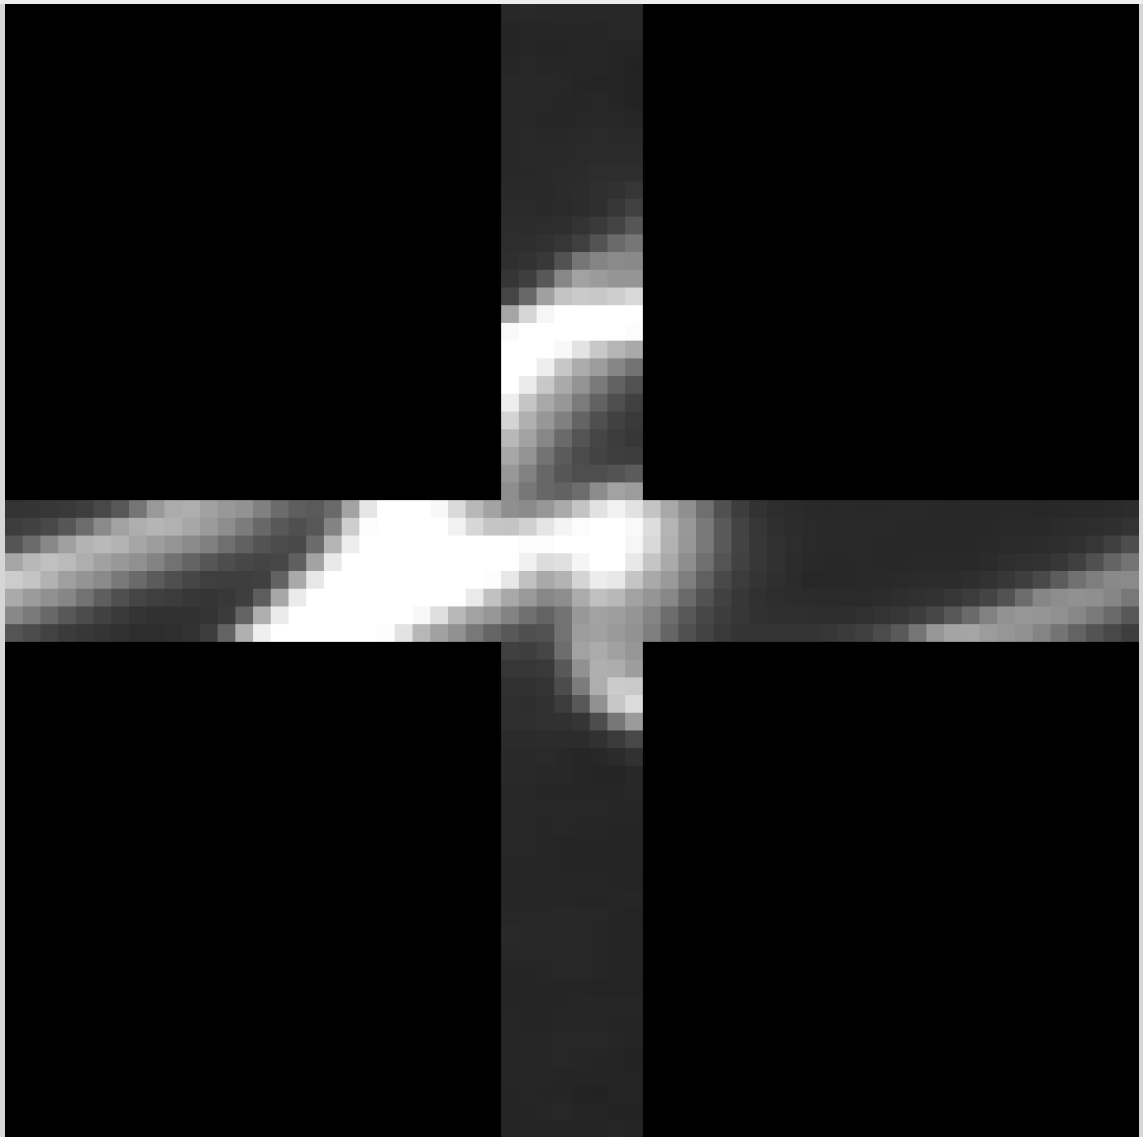
\includegraphics[width=4cm]{images/lrc_sample_inside.png}
		};
	\node[left=20mm of inner_inside,
		minimum height=5cm, 
		minimum width=5cm]
		(inner_outside)
		{
			
\includegraphics[width=4cm]{images/lrc_sample_outside.png}
		};
	\node[right=19mm of inner_inside,
		minimum height=5cm, 
		minimum width=5cm]
		(inner_intersects)
		{
			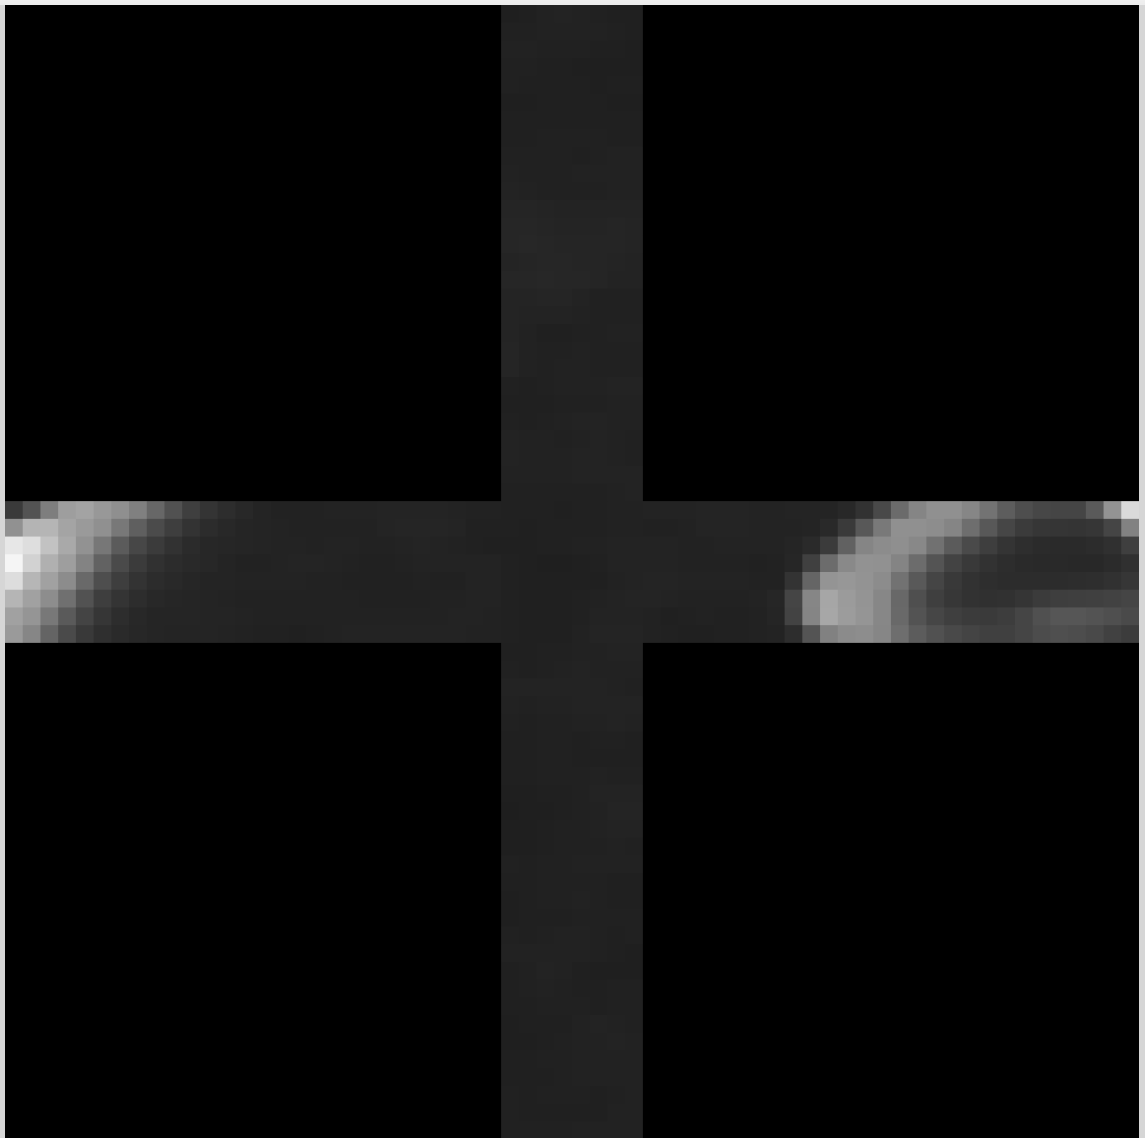
\includegraphics[width=4cm]{images/lrc_sample_intersects.png}
		};
		\node[above=-2mm of inner_inside]
		{
			\normalsize inside
		};
		\node[above=-2mm of inner_intersects]
		{
			\normalsize intersects
		};
		\node[above=-2mm of inner_outside]
		{
			\normalsize outside
		};
	\node[
	minimum height=5cm, 
	minimum width=5cm]
	at ([yshift=3.8em, xshift=0em] inside.south)
	(inner_inside)
	{
		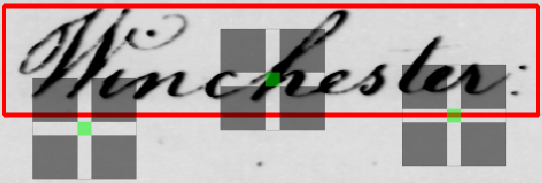
\includegraphics[width=20cm]{images/lrc_crossmask_label_example.png}
	};
	%%%%%%%%%%%%%%%%%%%%%%%%%%%%%%%%%%%%%%%%%%%%%%%%%%%%%%%%%%%%%%%%%%%%%%%%%%%%
	
	
	%%%%%%%%%%%%%%%%%%%%%%%%%%%%%%%%%%%%%%%%%%%%%%%%%%%%%%%%%%%%%%%%%%%%%%%%%%%%
	% 2. LRC architecture
	\node[
	line width=0.5mm,
	right=3cm of inside, 
	rounded corners=50pt, 
	rectangle, draw, 
	minimum height=17cm, 
	minimum width=22cm] 
	(lrc_net)
	{};
	\node[]
	at ([xshift=6.3em, yshift=-1em] lrc_net.north west)
	{
		\Large{2. Local Region Network}
	};
	\node[
	minimum height=5cm, 
	minimum width=5cm]
	at ([yshift=6em] lrc_net.south)
	{
		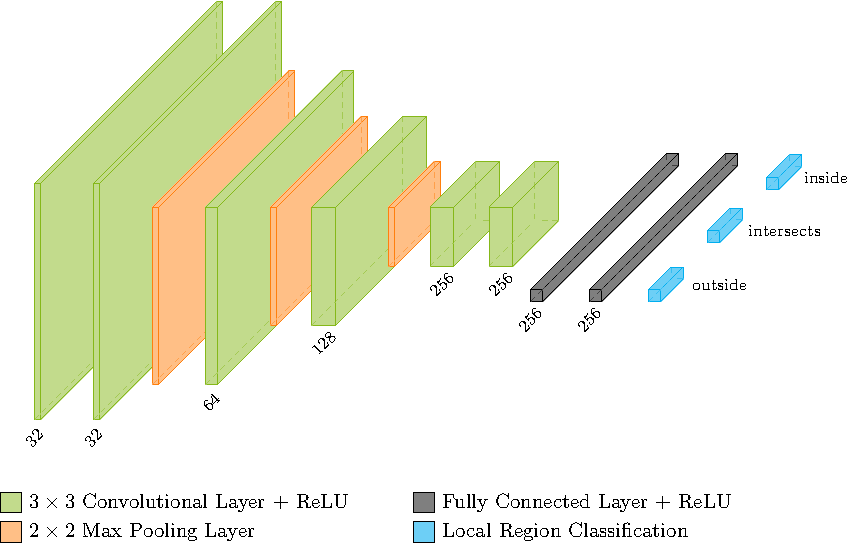
\includegraphics[width=20cm]{images/lrc_architecture-crop.pdf}
	};
	%%%%%%%%%%%%%%%%%%%%%%%%%%%%%%%%%%%%%%%%%%%%%%%%%%%%%%%%%%%%%%%%%%%%%%%%%%%%
	
	
	%%%%%%%%%%%%%%%%%%%%%%%%%%%%%%%%%%%%%%%%%%%%%%%%%%%%%%%%%%%%%%%%%%%%%%%%%%%%
	% 3. Text Detector Scores
	\node[
	line width=0.5mm,
	right=3cm of lrc_net, 
	rounded corners=50pt, 
	rectangle, draw, 
	minimum height=17cm, 
	minimum width=22cm] (lrc_example)
	{
	};
	\node[]
	at ([xshift=5em, yshift=-1em] lrc_example.north west)
	{
		\Large{3. Detection Scores}
	};
	\node[
	minimum height=5cm, 
	minimum width=5cm]
	at ([yshift=-7.3em] lrc_example.north)
	{
		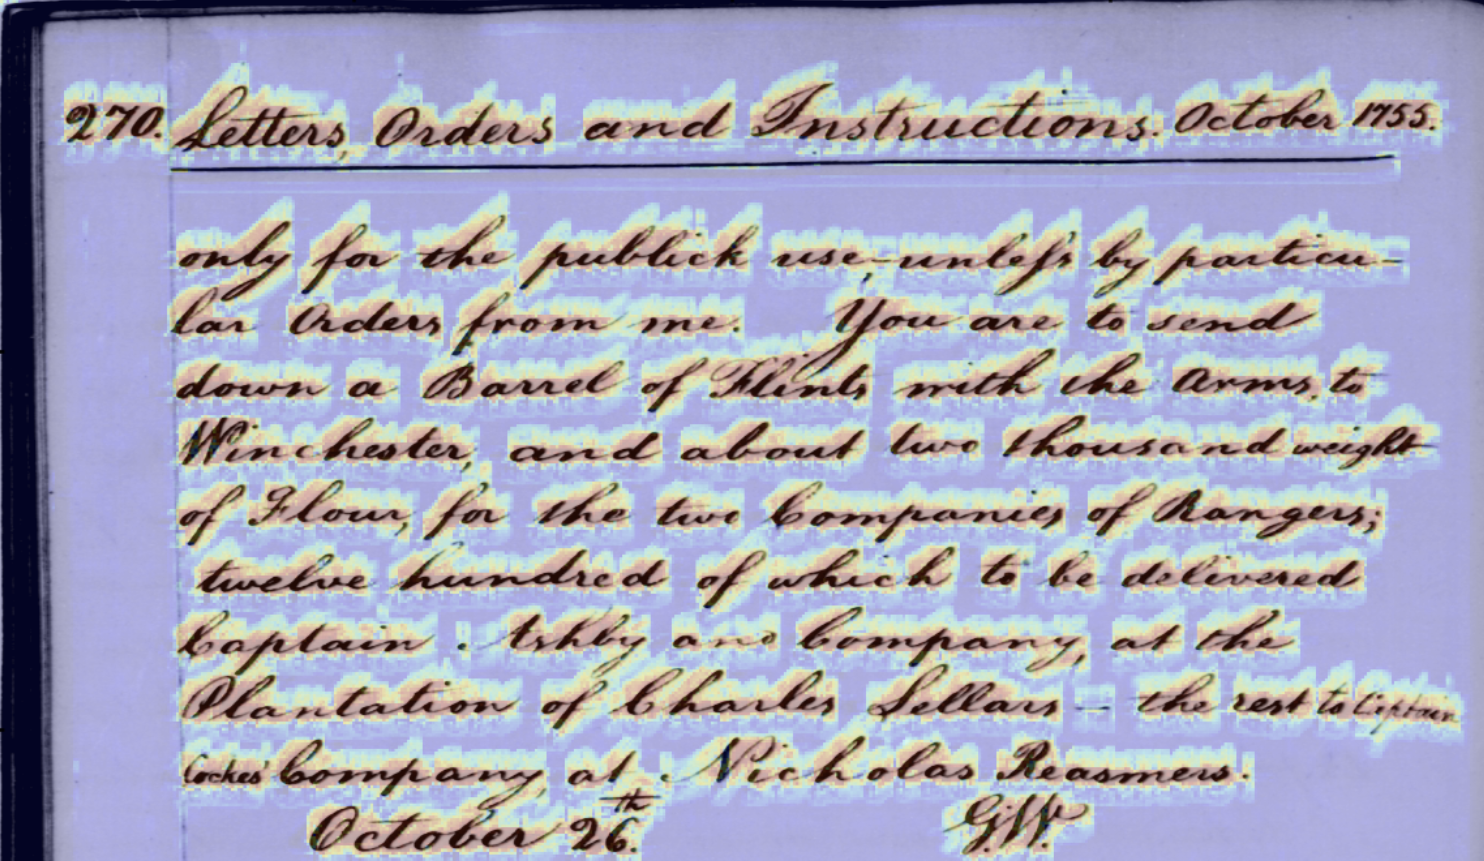
\includegraphics[width=20cm]{images/lrc_output_top.png}
	};
%	\node[
%	minimum height=5cm, 
%	minimum width=5cm,
%	text width=18cm,
%	text height=5cm]
%	at ([yshift=4.3em, xshift=0.6em] lrc_example.south)
%	(inner_inside)
%	{
%		\normalsize
%		Training samples cropped from the document inverted 
%		and masked 
%		by a cross shape.
%	};
	%%%%%%%%%%%%%%%%%%%%%%%%%%%%%%%%%%%%%%%%%%%%%%%%%%%%%%%%%%%%%%%%%%%%%%%%%%%%
	
	%%%%%%%%%%%%%%%%%%%%%%%%%%%%%%%%%%%%%%%%%%%%%%%%%%%%%%%%%%%%%%%%%%%%%%%%%%%%
	% 4. Word hypotheses
%	\node[
%	below=3cm of inside, 
%	rounded corners=50pt, 
%	rectangle, draw, 
%	minimum height=17cm, 
%	minimum width=22cm] 
%	(word_hypotheses)
%	{};
%	\node[]
%	at ([xshift=5.1em, yshift=-1em] word_hypotheses.north west)
%	{
%		\Large{4. Word hypotheses}
%	};
%	\node[ 
%	rounded corners=3pt, 
%	minimum height=5cm, 
%	minimum width=5cm]
%	at ([yshift=-7.3em, xshift=0em] word_hypotheses.north)
%	{
%		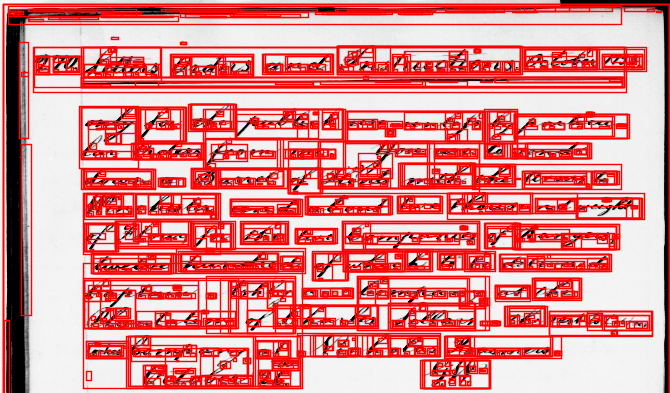
\includegraphics[width=20cm]{images/sift_regions_top.png}
%	};
	%%%%%%%%%%%%%%%%%%%%%%%%%%%%%%%%%%%%%%%%%%%%%%%%%%%%%%%%%%%%%%%%%%%%%%%%%%%%
	
	%%%%%%%%%%%%%%%%%%%%%%%%%%%%%%%%%%%%%%%%%%%%%%%%%%%%%%%%%%%%%%%%%%%%%%%%%%%%
	% 5. Matching
%	\node[
%	right=3cm of word_hypotheses, 
%	rounded corners=50pt, 
%	rectangle, draw, 
%	minimum height=17cm, 
%	minimum width=22cm] 
%	(matching)
%	{};
%	\node[]
%	at ([xshift=3.4em, yshift=-1em] matching.north west)
%	{
%		\Large{5. Matching}
%	};
%	\node[
%	rounded corners=20pt,
%	rectangle, draw,
%	minimum height=4cm, 
%	minimum width=0cm,
%	label=above:{\normalsize Query}]
%	(query)
%	at ([yshift=-70mm, xshift=45mm] matching.north)
%	{
%		
\includegraphics[height=2.5cm]{images/gw/query_by_string.png}
%		\hspace{0.1mm}
%		
\includegraphics[height=2.5cm]{images/gw/query_2700270_the_168.png}
%	};
%	\node[
%	rounded corners=20pt,
%	rectangle, draw,
%	align=center,
%	minimum height=4cm, 
%	minimum width=8cm,
%	label=above:{\normalsize Word Hypotheses}]
%	(phoc)
%	at ([yshift=-70mm, xshift=-60mm] matching.north)
%	{
%		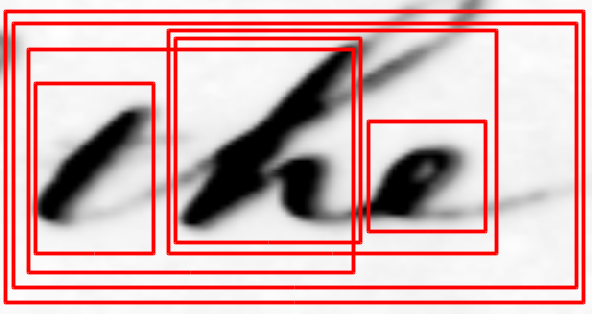
\includegraphics[height=3cm]{images/gw/query_the.png}
%	};
%	\node[
%	rounded corners=20pt,
%	ellipse, draw,
%	minimum height=0cm, 
%	minimum width=0cm]
%	(similarity)
%	at ([yshift=30mm, xshift=0mm] matching.south)
%	{
%		\large Matching
%	};
%	\node[
%	rounded corners=10pt,
%	rectangle, draw,
%	align=center,
%	minimum height=0cm, 
%	minimum width=0cm]
%	(nms)
%	at ([yshift=30mm, xshift=50mm] matching.south)
%	{
%		\large Non-Maximum \\
%		\large Suppression
%	};
%	
%	\draw[-stealth, line width=5pt] 
%	(query) -- (similarity) 
%	node[midway, anchor=west, outer sep=15pt, inner sep=5pt, fill=green!40] 
%	{\small PHOC};
%	
%	\draw[-stealth, line width=5pt] 
%	(phoc) -- (similarity) 
%	node[midway, anchor=east, outer sep=15pt, inner sep=5pt, fill=green!40] 
%	{\small PHOC};
	
%	\draw[-stealth, line width=5pt] 
%	(similarity) -- (nms)
%	node[]{}; 
	
	%%%%%%%%%%%%%%%%%%%%%%%%%%%%%%%%%%%%%%%%%%%%%%%%%%%%%%%%%%%%%%%%%%%%%%%%%%%%
	
	%%%%%%%%%%%%%%%%%%%%%%%%%%%%%%%%%%%%%%%%%%%%%%%%%%%%%%%%%%%%%%%%%%%%%%%%%%%%
	% 6. Retrieval Result
%	\node[
%	right=3cm of matching, 
%	rounded corners=50pt, 
%	rectangle, draw, 
%	minimum height=17cm, 
%	minimum width=22cm] 
%	(retrieval_result)
%	{};
%	\node[]
%	at ([xshift=4.9em, yshift=-1em] retrieval_result.north west)
%	{
%		\Large{6. Retrieval Result}
%	};
%	\node[ 
%	rounded corners=3pt, 
%	minimum height=5cm, 
%	minimum width=5cm]
%	at ([yshift=-7.3em, xshift=0em] retrieval_result.north)
%	{
%		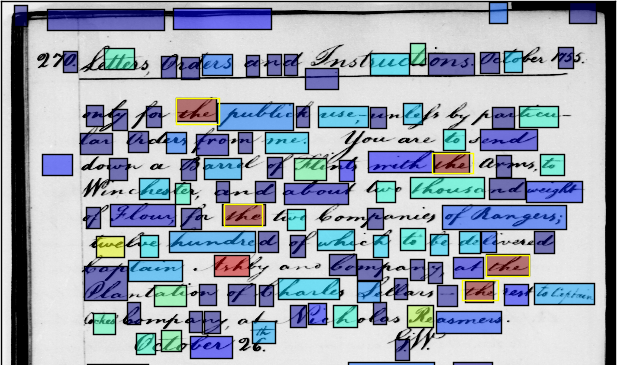
\includegraphics[width=20cm]{images/retrieval_the_top.png}
%	};
	%%%%%%%%%%%%%%%%%%%%%%%%%%%%%%%%%%%%%%%%%%%%%%%%%%%%%%%%%%%%%%%%%%%%%%%%%%%%
	
	
%	% Word hypotheses
%	\node[right=6cm of detector_scores, rounded corners=5pt, label=above:{5. Word hypotheses}, rectangle, draw, minimum height=17cm, minimum width=20cm] (ER-hyp)
%	{
%		\begin{tabular}{@{}c@{}}
%		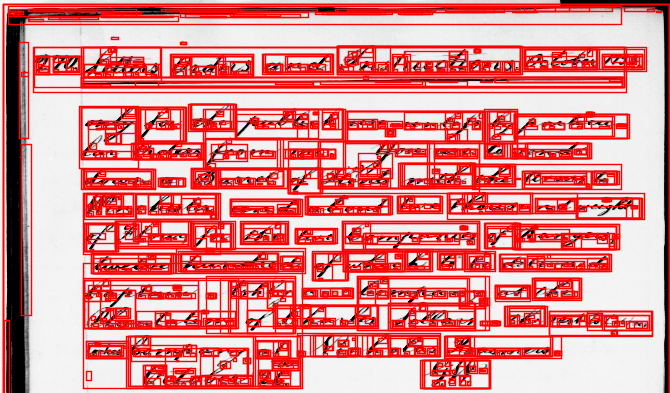
\includegraphics[width=19cm]{images/sift_regions_top.png}\\
%		\large{here comes some text}\\
%		\large{~}\\
%		\large{~}\\
%		\large{~}
%		\end{tabular}
%	};
%	% Retrieval results
%	\node[right=6cm of ER-hyp, rounded corners=5pt, label=above:{6. Retrieval result}, rectangle, draw, minimum height=20cm, minimum width=20cm, text ragged] (ret)
%	{
%		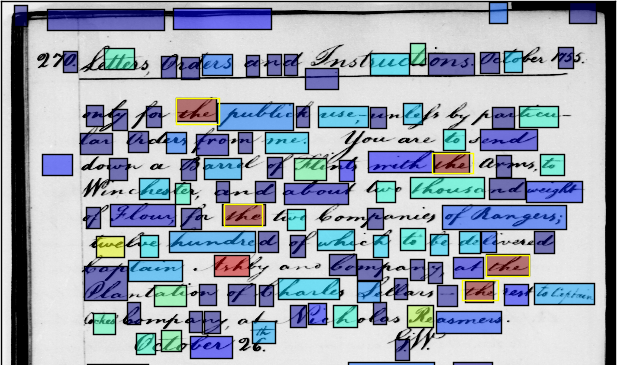
\includegraphics[width=19cm]{images/retrieval_the_top.png}
%	};

	
	%Query
%	\node[node distance=5cm, below=of SIFT, rounded corners=5pt, minimum width=10cm, label=above:{Query}, draw](Query)
%	{
%		
\includegraphics[height=4cm, frame]{images/gw/query_by_string.png}
%		\hspace{1em}
%		
\includegraphics[height=4cm, frame]{images/gw/query_2700270_the_168.png}
%	};
	
%	\node[ellipse, minimum height=4cm, minimum width=10cm, xshift=3cm, draw](SIM) at (Query -| ER-hyp) {\Large Similarity};
%	
%	\node[rectangle, minimum height=7cm, text width=8.5cm, draw](NMS) at (SIM -| ret) {\Large Non-maximum suppression};
%	
%	\node[above=1cm of SIM, triangle, border rotated, inner sep=15pt, draw](AR){};
	
%	\draw[-stealth, line width=5pt] (Query) -- (SIM) node[midway, anchor=north, outer sep=10pt, inner sep=5pt, fill=green!20] {PHOC}; 
%	\draw[line width=5pt] (ER-hyp.south -| AR) -- (AR) node[midway, anchor=west, outer sep=10pt, inner sep=5pt, fill=green!20] {PHOC};
%	\draw[-stealth, line width=5pt] (AR) -- (SIM); 
%	\draw[-stealth, line width=5pt] (SIM) -- (NMS) -- (ret); 
%	\draw[dashed, line width=3pt] (Query.north east) -- (Query.north east |- AR) -- (AR) node [midway, anchor=south]{Aspect ratio filter};
%	\draw[-stealth, line width=5pt] (SIFT) -- (ER-hyp);
\end{tikzpicture}
%\end{center}
\vspace*{-10mm}

\postersection{System Context}

\begin{tikzpicture}[
	node distance = 5cm,
	%nodes=draw,
	auto,
	scale=1.0,
	transform shape,
	triangle/.style = {regular polygon, regular polygon sides=3 },
    node rotated/.style = {rotate=180},
    border rotated/.style = {shape border rotate=180}
	]
	
		%%%%%%%%%%%%%%%%%%%%%%%%%%%%%%%%%%%%%%%%%%%%%%%%%%%%%%%%%%%%%%%%%%%%%%%%%%%%
	% 4. Word hypotheses
	\node[ 
	line width=0.5mm,
	rounded corners=50pt, 
	rectangle, draw, 
	minimum height=17cm, 
	minimum width=22cm]
	at (0,0) 
	(word_hypotheses)
	{};
	\node[]
	at ([xshift=5.1em, yshift=-1em] word_hypotheses.north west)
	{
		\Large{4. Word hypotheses}
	};
	\node[ 
	rounded corners=3pt, 
	minimum height=5cm, 
	minimum width=5cm]
	at ([yshift=-7.3em, xshift=0em] word_hypotheses.north)
	{
		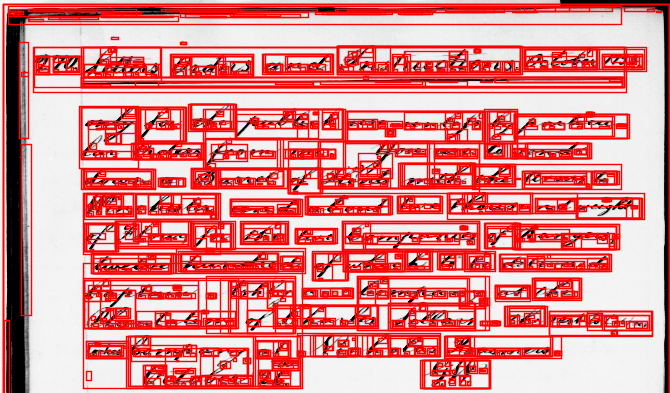
\includegraphics[width=20cm]{images/sift_regions_top.png}
	};
	%%%%%%%%%%%%%%%%%%%%%%%%%%%%%%%%%%%%%%%%%%%%%%%%%%%%%%%%%%%%%%%%%%%%%%%%%%%%
	
	%%%%%%%%%%%%%%%%%%%%%%%%%%%%%%%%%%%%%%%%%%%%%%%%%%%%%%%%%%%%%%%%%%%%%%%%%%%%
	% 5. Matching
	\node[
	line width=0.5mm,
	right=3cm of word_hypotheses, 
	rounded corners=50pt, 
	rectangle, draw, 
	minimum height=17cm, 
	minimum width=22cm] 
	(matching)
	{};
	\node[]
	at ([xshift=3.4em, yshift=-1em] matching.north west)
	{
		\Large{5. Matching}
	};
	\node[
	rounded corners=20pt,
	rectangle, draw,
	minimum height=4cm, 
	minimum width=0cm,
	label=above:{\normalsize Query}]
	(query)
	at ([yshift=-60mm, xshift=45mm] matching.north)
	{
		
\includegraphics[height=2.5cm]{images/gw/query_by_string.png}
		\hspace{0.1mm}
		
\includegraphics[height=2.5cm]{images/gw/query_2700270_the_168.png}
	};
	\node[
	rounded corners=20pt,
	rectangle, draw,
	align=center,
	minimum height=4cm, 
	minimum width=8cm,
	label=above:{\normalsize Word Hypotheses}]
	(phoc)
	at ([yshift=-60mm, xshift=-60mm] matching.north)
	{
		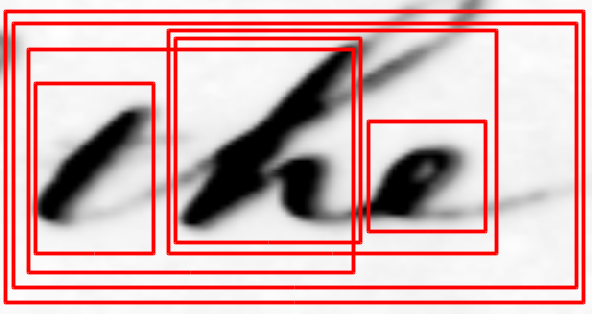
\includegraphics[height=3cm]{images/gw/query_the.png}
	};
	\node[
	rounded corners=20pt,
	circle, draw,
	fill=red!20!green,
	minimum height=0cm, 
	minimum width=0cm]
	(similarity)
	at ([yshift=40mm, xshift=0mm] matching.south)
	{
		\large Matching
	};
%	\node[
%	rounded corners=10pt,
%	rectangle, draw,
%	align=center,
%	minimum height=0cm, 
%	minimum width=0cm]
%	(nms)
%	at ([yshift=30mm, xshift=50mm] matching.south)
%	{
%		\large Non-Maximum \\
%		\large Suppression
%	};
	
	\draw[-stealth, line width=5pt] 
	(query) -- (similarity) 
	node[midway, anchor=west, outer sep=15pt, inner sep=5pt, fill=green!40] 
	{\small PHOC};
	
	\draw[-stealth, line width=5pt] 
	(phoc) -- (similarity) 
	node[midway, anchor=east, outer sep=15pt, inner sep=5pt, fill=green!40] 
	{\small PHOC};
	
%	\draw[-stealth, line width=5pt] 
%	(similarity) -- (nms)
%	node[]{}; 
	
	%%%%%%%%%%%%%%%%%%%%%%%%%%%%%%%%%%%%%%%%%%%%%%%%%%%%%%%%%%%%%%%%%%%%%%%%%%%%
	
	%%%%%%%%%%%%%%%%%%%%%%%%%%%%%%%%%%%%%%%%%%%%%%%%%%%%%%%%%%%%%%%%%%%%%%%%%%%%
	% 6. Retrieval Result
	\node[
	line width=0.5mm,
	right=3cm of matching, 
	rounded corners=50pt, 
	rectangle, draw, 
	minimum height=17cm, 
	minimum width=22cm] 
	(retrieval_result)
	{};
	\node[]
	at ([xshift=4.9em, yshift=-1em] retrieval_result.north west)
	{
		\Large{6. Retrieval Result}
	};
	\node[ 
	rounded corners=3pt, 
	minimum height=5cm, 
	minimum width=5cm]
	at ([yshift=-7.3em, xshift=0em] retrieval_result.north)
	{
		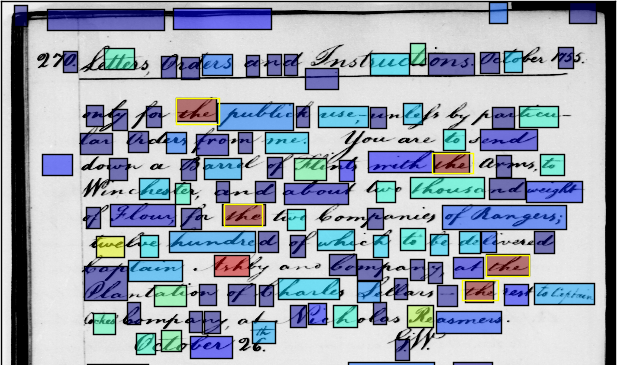
\includegraphics[width=20cm]{images/retrieval_the_top.png}
	};
	%%%%%%%%%%%%%%%%%%%%%%%%%%%%%%%%%%%%%%%%%%%%%%%%%%%%%%%%%%%%%%%%%%%%%%%%%%%%
	
\end{tikzpicture}

\postersection{Future Research}
%\vspace*{-10mm}
\begin{tikzpicture}[
	node distance = 5cm,
	%nodes=draw,
	auto,
	scale=1.0,
	transform shape,
	triangle/.style = {regular polygon, regular polygon sides=3 },
    node rotated/.style = {rotate=180},
    border rotated/.style = {shape border rotate=180}
	]
	
	\node[
	rounded corners=50pt,  
	%rectangle, draw, 
	minimum height=10cm, 
	minimum width=10cm,
	] 
	(natural_text)
	at (0,0)
	{	};
	\node[ 
	rounded corners=3pt, 
	minimum height=0cm, 
	minimum width=0cm,
	label=above:{Historical Document}]
	(histo)
	at ([yshift=+50mm, xshift=0em] natural_text.center)
	{
		
\includegraphics[width=14cm]{images/future_research_gw.png}
	};
	
	\node[
	rounded corners=3pt, 
	minimum height=0cm, 
	minimum width=0cm,
	label=above:{Natural Scene Text}]
	at ([yshift=-50mm, xshift=0em] natural_text.center)
	{
		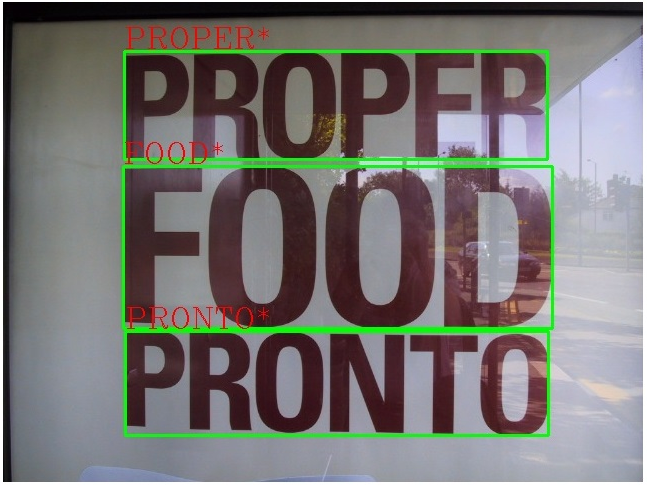
\includegraphics[width=7cm]{images/natural_scene_text.png}
	};
	
	\node[
	right=5cm of natural_text, 
	rounded corners=50pt, 
	%rectangle, draw, 
	minimum height=17cm, 
	minimum width=31cm]
	%label=above:{PHOCnet\normalsize[2]}] 
	(phoc_net)
	{};
	\node[ 
	rounded corners=3pt, 
	minimum height=5cm, 
	minimum width=5cm]
	at ([yshift=0mm, xshift=0em] phoc_net.center)
	{
		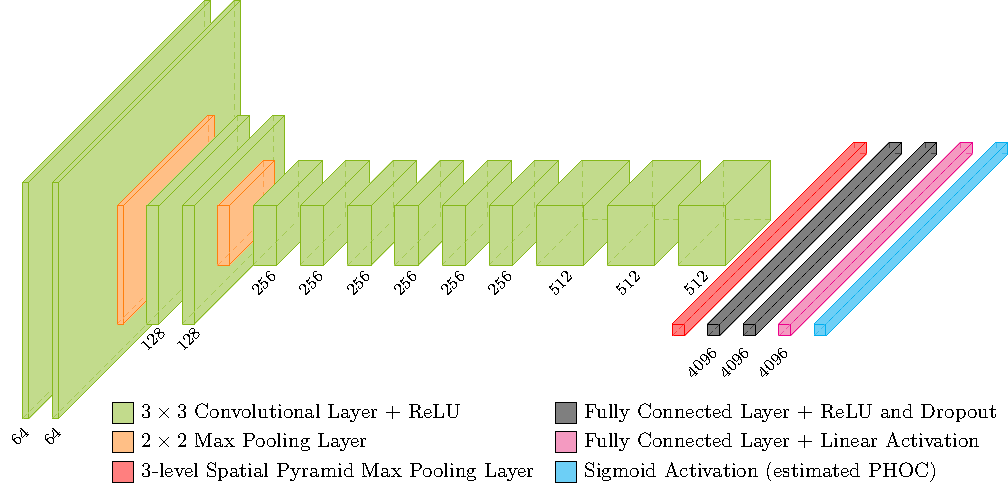
\includegraphics[width=35cm]{images/aam-phocnet-architecture.pdf}
	};
	
	\node[
	right=3cm of phoc_net, 
	rounded corners=50pt, 
	%rectangle, draw, 
	minimum height=17cm, 
	minimum width=18.7cm] 
	(lexicon_matching)
	{};
	\node[
	rounded corners=10pt,
	rectangle, draw,
	align=left,
	minimum height=4cm, 
	minimum width=0cm,
	label=above:{Lexicon}]
	(lexicon)
	at ([yshift=0mm, xshift=-33mm] lexicon_matching.east)
	{
		\texttt{\normalsize~} \\
		\texttt{[proper]} \\
		\texttt{[letters]} \\
		\texttt{[the]} \\
		\texttt{[commander]} \\
		\texttt{[food]} \\
		\texttt{[winchester]} \\
		\texttt{[...]}\\
		\texttt{\normalsize~}
	};
	\node[
	left=4cm of lexicon,
	rounded corners=20pt,
	circle, draw,
	minimum height=0cm, 
	minimum width=0cm,
	fill=red!20!green]
	(matching)
	%at ([yshift=30mm, xshift=0mm] lexicon_matching.south)
	{
		\large Matching
	};
	
	\draw[-stealth, line width=5pt] 
	(phoc_net) -- (matching) 
	node[midway, anchor=north, outer sep=15pt, inner sep=5pt, fill=green!40] 
	{\small PHOC};
	
	\draw[-stealth, line width=5pt] 
	(lexicon) -- (matching) 
	node[midway, anchor=north, outer sep=15pt, inner sep=5pt, fill=green!40] 
	{\small PHOC};	
	
\end{tikzpicture}
	
%\vspace*{-20mm}

\section*{\sf \textbf{References}}
\normalsize
\begin{itemize}[leftmargin=1.35em]
 \item[{[1]}] L. Rothacker, S. Sudholt, E. Rusakov, 
 M. Kasperidusa and G. A. Fink, "Word Hypotheses for Segmentation-free Word Spotting 
 in Historic Document Images", in {\em Document Analysis and Recognition (ICDAR)}, 2017
  
  \item[{[2]}] S. Sudholt and G. A. Fink, "PHOCNet: A Deep Convolutional Neural Network
  for Word Spotting in Handwritten Documents, in {\em International Conference on 
  Frontiers in Handwritting Recognition}, 2016, pp. 277-282

\end{itemize}

\end{document}